% Generated by plsimcount.pfseeds -- do not edit; regenerate instead.
% figure: A-measured-by-order -- Suzuki formulas of each order, r from: Measured $r$; median over seeds [1, 2, 3, 4, 5], bars = min..max
% metric=cnot gatebase=cz merged
% seed 1: git_commit=04cd66abb614bdc66fb48e891cef085a299e0ab1 git_dirty=False
% seed 2: git_commit=04cd66abb614bdc66fb48e891cef085a299e0ab1 git_dirty=False
% seed 3: git_commit=04cd66abb614bdc66fb48e891cef085a299e0ab1 git_dirty=False
% seed 4: git_commit=04cd66abb614bdc66fb48e891cef085a299e0ab1 git_dirty=False
% seed 5: git_commit=04cd66abb614bdc66fb48e891cef085a299e0ab1 git_dirty=False
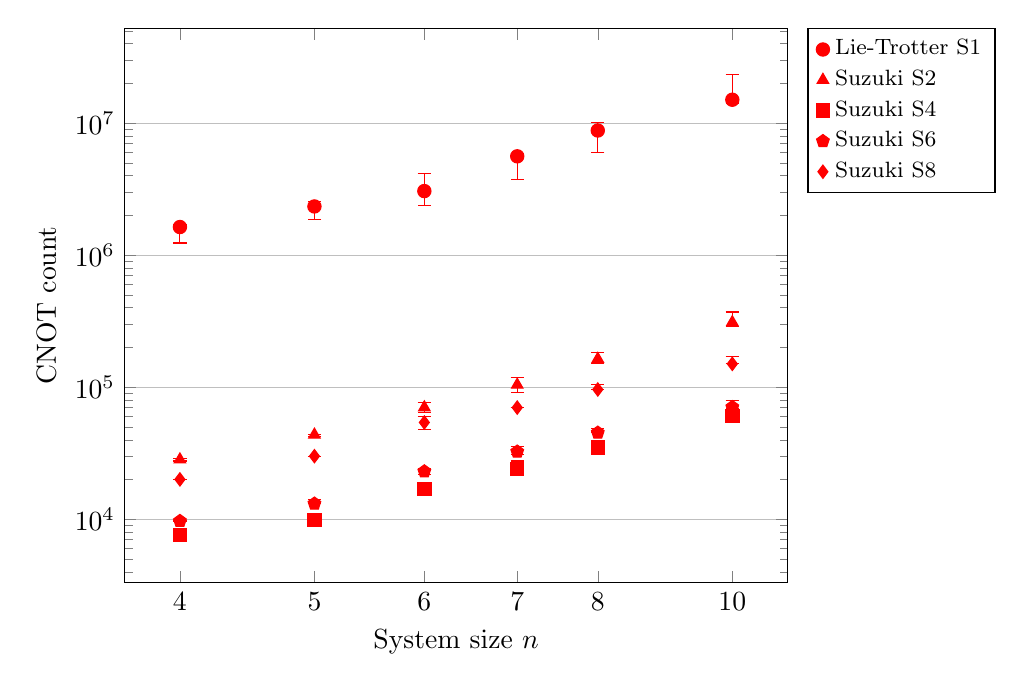
\begin{tikzpicture}
  \begin{loglogaxis}[
    width=10cm,
    xlabel={System size $n$},
    ylabel={CNOT count},
    xtick={4,5,6,7,8,10},
    xticklabels={4,5,6,7,8,10},
    ymajorgrids=true,
    legend pos=outer north east,
    legend cell align=left,
    legend style={font=\footnotesize},
  ]
    \addplot[only marks, red, mark=*, mark size=2.4pt, mark options={solid, fill=red}, error bars/.cd, y dir=both, y explicit, error bar style={red}] coordinates {
      (4,1635000) += (0,58872) -= (0,398232)
      (5,2340870) += (0,193320) -= (0,484950)
      (6,3061044) += (0,1067832) -= (0,692676)
      (7,5613468) += (0,289128) -= (0,1857954)
      (8,8806032) += (0,1371216) -= (0,2842320)
      (10,15058080) += (0,8352240) -= (0,1020540)
    };
    \addlegendentry{Lie-Trotter S1}
    \addplot[only marks, red, mark=triangle*, mark size=2.4pt, mark options={solid, fill=red}, error bars/.cd, y dir=both, y explicit, error bar style={red}] coordinates {
      (4,28320) += (0,360) -= (0,680)
      (5,43650) += (0,400) -= (0,1550)
      (6,70260) += (0,6660) -= (0,5400)
      (7,104300) += (0,14770) -= (0,13580)
      (8,163680) += (0,18960) -= (0,12320)
      (10,310300) += (0,61400) -= (0,22300)
    };
    \addlegendentry{Suzuki S2}
    \addplot[only marks, red, mark=square*, mark size=2.4pt, mark options={solid, fill=red}, error bars/.cd, y dir=both, y explicit, error bar style={red}] coordinates {
      (4,7560) += (0,168) -= (0,168)
      (5,9870) += (0,1260) -= (0,420)
      (6,16884) += (0,1008) -= (0,1008)
      (7,24108) += (0,3528) -= (0,1470)
      (8,34944) += (0,2352) -= (0,1008)
      (10,60480) += (0,6720) -= (0,1680)
    };
    \addlegendentry{Suzuki S4}
    \addplot[only marks, red, mark=pentagon*, mark size=2.4pt, mark options={solid, fill=red}, error bars/.cd, y dir=both, y explicit, error bar style={red}] coordinates {
      (4,9696) += (0,0) -= (0,0)
      (5,13130) += (0,1010) -= (0,0)
      (6,23028) += (0,1212) -= (0,1212)
      (7,32522) += (0,2828) -= (0,1414)
      (8,45248) += (0,3232) -= (0,0)
      (10,70700) += (0,8080) -= (0,2020)
    };
    \addlegendentry{Suzuki S6}
    \addplot[only marks, red, mark=diamond*, mark size=2.4pt, mark options={solid, fill=red}, error bars/.cd, y dir=both, y explicit, error bar style={red}] coordinates {
      (4,20040) += (0,0) -= (0,0)
      (5,30060) += (0,0) -= (0,0)
      (6,54108) += (0,6012) -= (0,6012)
      (7,70140) += (0,0) -= (0,0)
      (8,96192) += (0,8016) -= (0,0)
      (10,150300) += (0,20040) -= (0,0)
    };
    \addlegendentry{Suzuki S8}
  \end{loglogaxis}
\end{tikzpicture}
